\documentclass[tikz,border=8pt]{standalone}
\usepackage[utf8]{inputenc}
\usepackage{lmodern}
\usepackage[T1]{fontenc}
\usepackage{amsmath,amssymb}
\usetikzlibrary{shapes.geometric, arrows.meta, positioning, calc, fit, backgrounds}

\definecolor{orangeA}{HTML}{C2410C}
\definecolor{orangeB}{HTML}{EA580C}
\definecolor{orangeC}{HTML}{FFF7ED}
\definecolor{blueA}{HTML}{1D4ED8}
\definecolor{blueB}{HTML}{3B82F6}
\definecolor{blueC}{HTML}{EFF6FF}
\definecolor{cyanA}{HTML}{0E7490}
\definecolor{cyanC}{HTML}{ECFEFF}
\definecolor{greenA}{HTML}{15803D}
\definecolor{greenC}{HTML}{F0FDF4}
\definecolor{slateG}{HTML}{475569}
\definecolor{amberA}{HTML}{D97706}
\definecolor{amberC}{HTML}{FEF3C7}

\begin{document}
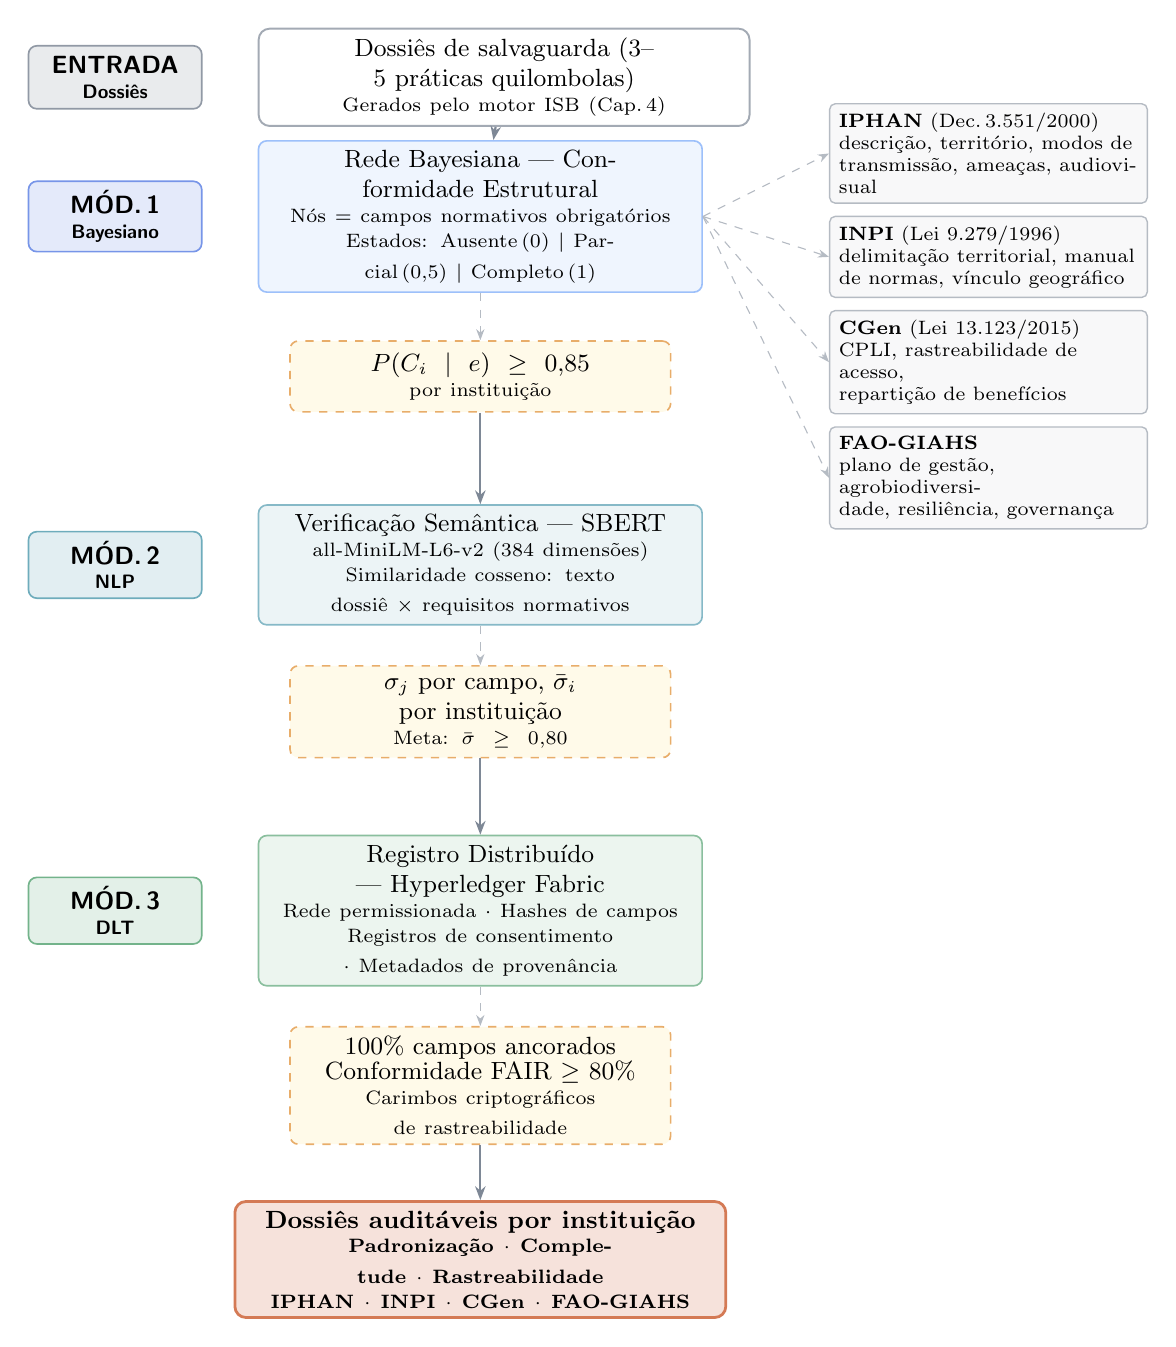
\begin{tikzpicture}[
  phase/.style={
    fill=#1!12, draw=#1!60,
    font=\sffamily\bfseries\small,
    minimum width=2.2cm, minimum height=0.8cm,
    align=center, rounded corners=3pt,
    line width=0.6pt
  },
  mainbox/.style={
    draw=slateG!50, fill=white,
    font=\small, align=center,
    minimum width=6.2cm, minimum height=1.0cm,
    rounded corners=4pt, text width=6.0cm,
    line width=0.7pt
  },
  modbox/.style={
    draw=#1!50, fill=#1!8,
    font=\small, align=center,
    minimum width=5.6cm, minimum height=0.9cm,
    rounded corners=3pt, text width=5.4cm,
    line width=0.6pt
  },
  metricbox/.style={
    draw=amberA!60, fill=amberC!40,
    font=\small, align=center,
    minimum width=4.8cm, minimum height=0.9cm,
    rounded corners=3pt, text width=4.6cm,
    line width=0.6pt, dashed
  },
  outputbox/.style={
    draw=#1!70, fill=#1!15,
    font=\small\bfseries, align=center,
    minimum width=6.2cm, minimum height=1.0cm,
    rounded corners=4pt, text width=6.0cm,
    line width=1pt
  },
  instbox/.style={
    draw=slateG!40, fill=slateG!4,
    font=\scriptsize, align=left,
    minimum width=4.0cm, minimum height=0.7cm,
    rounded corners=2pt, text width=3.8cm,
    line width=0.5pt
  },
  arr/.style={-{Stealth[length=5pt]}, thick, slateG!70},
  darr/.style={-{Stealth[length=4pt]}, thin, slateG!40, dashed},
  node distance=0.55cm
]

%% ═══ ENTRADA ═══
\node[phase=slateG] (ph0) {ENTRADA\\[-2pt]{\scriptsize Dossi\^es}};

\node[mainbox, right=0.7cm of ph0] (input)
  {Dossi\^es de salvaguarda (3--5 pr\'aticas quilombolas)\\[-2pt]
   {\scriptsize Gerados pelo motor ISB (Cap.\,4)}};

%% ═══ MÓDULO 1 — REDE BAYESIANA ═══
\node[phase=blueA, below=0.9cm of ph0] (ph1)
  {M\'OD.\,1\\[-2pt]{\scriptsize Bayesiano}};

\node[modbox=blueB, right=0.7cm of ph1] (bn)
  {Rede Bayesiana --- Conformidade Estrutural\\[-2pt]
   {\scriptsize N\'os = campos normativos obrigat\'orios}\\[-2pt]
   {\scriptsize Estados: Ausente\,(0) $\mid$ Parcial\,(0{,}5) $\mid$ Completo\,(1)}};
\draw[arr] (input) -- (bn);

%% Instituições (à direita)
\node[instbox, right=1.6cm of bn, yshift=0.8cm] (iphan)
  {\textbf{IPHAN} (Dec.\,3.551/2000)\\
   descri\c{c}\~ao, territ\'orio, modos de\\
   transmiss\~ao, amea\c{c}as, audiovisual};

\node[instbox, below=0.15cm of iphan] (inpi)
  {\textbf{INPI} (Lei 9.279/1996)\\
   delimita\c{c}\~ao territorial, manual\\
   de normas, v\'{\i}nculo geogr\'afico};

\node[instbox, below=0.15cm of inpi] (cgen)
  {\textbf{CGen} (Lei 13.123/2015)\\
   CPLI, rastreabilidade de acesso,\\
   reparti\c{c}\~ao de benef\'{\i}cios};

\node[instbox, below=0.15cm of cgen] (fao)
  {\textbf{FAO-GIAHS}\\
   plano de gest\~ao, agrobiodiversi-\\
   dade, resili\^encia, governan\c{c}a};

\draw[darr] (bn.east) -- (iphan.west);
\draw[darr] (bn.east) -- (inpi.west);
\draw[darr] (bn.east) -- (cgen.west);
\draw[darr] (bn.east) -- (fao.west);

\node[metricbox, below=0.6cm of bn] (mbn)
  {$P(C_i \mid e) \geq 0{,}85$\\[-2pt]
   {\scriptsize por institui\c{c}\~ao}};
\draw[darr] (bn) -- (mbn);

%% ═══ MÓDULO 2 — SBERT ═══
\node[phase=cyanA, below=1.5cm of ph1 |- mbn.south] (ph2)
  {M\'OD.\,2\\[-2pt]{\scriptsize NLP}};

\node[modbox=cyanA, right=0.7cm of ph2] (sbert)
  {Verifica\c{c}\~ao Sem\^antica --- SBERT\\[-2pt]
   {\scriptsize all-MiniLM-L6-v2 (384 dimens\~oes)}\\[-2pt]
   {\scriptsize Similaridade cosseno: texto dossi\^e $\times$ requisitos normativos}};
\draw[arr] (mbn) -- (sbert);

\node[metricbox, below=0.5cm of sbert] (msbert)
  {$\sigma_j$ por campo, $\bar{\sigma}_i$ por institui\c{c}\~ao\\[-2pt]
   {\scriptsize Meta: $\bar{\sigma} \geq 0{,}80$}};
\draw[darr] (sbert) -- (msbert);

%% ═══ MÓDULO 3 — DLT ═══
\node[phase=greenA, below=1.5cm of ph2 |- msbert.south] (ph3)
  {M\'OD.\,3\\[-2pt]{\scriptsize DLT}};

\node[modbox=greenA, right=0.7cm of ph3] (dlt)
  {Registro Distribu\'{\i}do --- Hyperledger Fabric\\[-2pt]
   {\scriptsize Rede permissionada $\cdot$ Hashes de campos}\\[-2pt]
   {\scriptsize Registros de consentimento $\cdot$ Metadados de proven\^ancia}};
\draw[arr] (msbert) -- (dlt);

\node[metricbox, below=0.5cm of dlt] (mdlt)
  {100\% campos ancorados\\[-2pt]
   Conformidade FAIR $\geq$ 80\%\\[-2pt]
   {\scriptsize Carimbos criptogr\'aficos de rastreabilidade}};
\draw[darr] (dlt) -- (mdlt);

%% ═══ SAÍDA ═══
\node[outputbox=orangeA, below=0.7cm of mdlt] (out)
  {Dossi\^es audit\'aveis por institui\c{c}\~ao\\[-2pt]
   {\scriptsize Padroniza\c{c}\~ao $\cdot$ Completude $\cdot$ Rastreabilidade}\\[-2pt]
   {\scriptsize IPHAN $\cdot$ INPI $\cdot$ CGen $\cdot$ FAO-GIAHS}};
\draw[arr] (mdlt) -- (out);

\end{tikzpicture}
\end{document}
